\section{Certificato Digitale}

Nella crittografia asimmetrica un \textbf{certificato digitale} è un
documento elettronico che attesta
l'associazione univoca tra una chiave pubblica e l'identità di un soggetto.
Il certificato digitale contiene informazioni sulla chiave,
sull'identità del proprietario
(denominato soggetto) e sulla firma digitale di un'entità che ha verificato
i contenuti del certificato
(denominato emittente) e riconosciuta come \textbf{CA}
(\textit{Certification Authority}).
Tale certificato, infatti, è
a sua volta autenticato per evitarne la falsificazione, sempre attraverso
firma digitale, ovvero viene
cifrato con la chiave privata dell'associazione, la quale fornisce poi la
rispettiva chiave pubblica per
verificarlo.
Ad una CA sono assegnati 10 compiti:
\begin{enumerate}
    \item Identificare con certezza la persona che fa richiesta della certificazione della chiave
          pubblica;
    \item Rilasciare e rendere pubblico il certificato;
    \item Garantire l'accesso telematico al registro delle chiavi pubbliche;
    \item Informare i richiedenti sulla procedura di certificazione;
    \item Dichiarare la propria politica di sicurezza;
    \item Attenersi alle norme sul trattamento di dati personali;
    \item Non rendersi depositario delle chiavi private;
    \item Procedere alla revoca o alla sospensione dei certificati in caso di richiesta dell'interessato o
          venendo a conoscenza di abusi o falsificazioni, ecc;
    \item Rendere pubblica la revoca o la sospensione delle chiavi;
    \item Assicurare la corretta manutenzione del sistema di certificazione.
\end{enumerate}

\subsection{Formato x.509}

Il formato più comune per i certificati di chiave pubblica è definito da X.509, raccomandato dalla
ITU (International Telecommunication Union).
Il certificato viene firmato da chi lo emette. “Codice identificativo
dell'emittente” è univoco per ogni
CA esistente. La firma garantisce il fatto che il documento è autentico,
cioè che è stato scritto dal
“nome soggetto” e che è stato verificato da “ente emettitore”.
E' importante specificare il “periodo di validità” poiché la stessa firma
(e la coppia chiave
pubblica-privata) ha una validità temporale. Se questa dovesse scadere,
il certificato va riemesso.
Ciò viene fatto anche nel momento in cui i ruoli (specificati nel campo
“estensioni”) di chi partecipa
alla sottoscrizione cambiano.
Viene anche specificato l'elenco degli algoritmi utilizzati per
l'apposizione della firma con i relativi
parametri.

\begin{figure}[H]
    \centering
    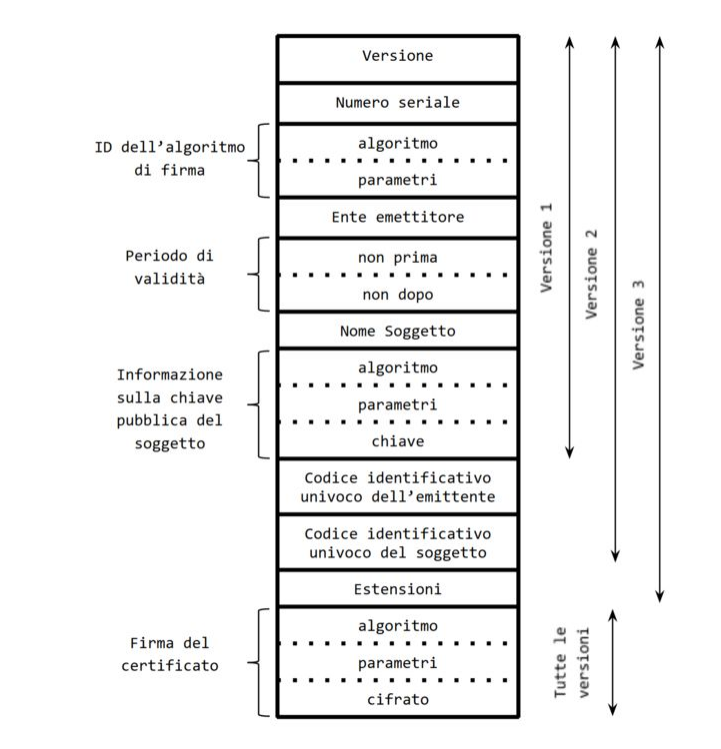
\includegraphics[width=10cm, keepaspectratio]{capitoli/crittografia/imgs/x509.png}
\end{figure}

\subsection{Ottenere un certificato Digitale}

Sono richieste le seguenti fasi: l'utente genera sul proprio PC una coppia
di chiavi. I browser
comuni offrono tale il servizio; la chiave privata è memorizzata localmente
in un file nascosto. Per
avere una maggiore sicurezza si potrebbero memorizzare le chiavi su una
SmartCard protetta da
un PIN. L'utente invia alla CA una richiesta di certificato, insieme alla
chiave pubblica generata; la
CA autentica il richiedente, di solito chiedendogli di recarsi di persona
ad uno sportello di \textbf{LVP}
(\textit{Local Validation Point}) collegato con la CA.
A questo punto, verificata l'identità, la CA emette il certificato,
lo invia al richiedente tramite posta
elettronica ed inserisce la chiave certificata nel registro delle chiavi
pubbliche.
L'intera procedura sopra descritta accade nell'ambito di una \textbf{PKI}
(\textit{Public Key Infrastructure}), la cui
struttura minima prevede la presenza di una CA ed un LVP; in generale
sono ammessi più LVP.
Una PKI può avere una struttura gerarchica in cui alcune CA certificano
altre CA, ottenendo una
“catena di fiducia”. Secondo tale struttura: la “Root CA” certifica le
CA di primo livello; le CA di
primo livello certificano le CA di secondo livello; le CA di ultimo
livello certificano il singolo utente.

\subsection{Revoca del certificato}

Il certificato può essere revocato per varie ragioni: cambio dei dati
personali (email, recapito, ecc),
licenziamento, dimissioni, Compromissione della chiave privata, ecc.
Può avvenire anche su richiesta da parte dell'utente o dell'emettitore.

\subsection{Certificate Revocation List}

Un \textbf{CRL} è un elenco di certificati digitali che sono stati revocati
dalla CA,
prima della data di scadenza pianificata e non dovrebbero più essere
considerati attendibili.
Viene generato e pubblicato periodicamente, spesso ad un intervallo di
tempo definito. Ad ogni
pubblicazione, infatti, viene anche comunicata la data del successivo
aggiornamento.
Viene rilasciato da un'entità autorizzata che è tipicamente la CA
che ha anche rilasciato i certificati
corrispondenti.

\begin{figure}[H]
    \centering
    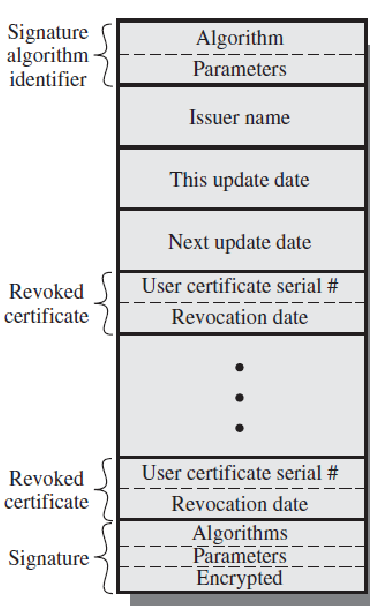
\includegraphics[width=4cm, keepaspectratio]{capitoli/crittografia/imgs/CRL.png}
\end{figure}